\chapter{Архитектура Evergrid}

\section{Основные ограничения}

В моем понимании проектирование архитектуры основывается на:

\begin{itemize}
	\item достаточно подробной постановке задачи
	\item выявлении ограничений
	\item использовании актуальных технологий как составных блоков
	\item бритве Оккама (не переусложняй!)
\end{itemize}

Постановка задачи у нас есть, последние два пункта постараемся соблюдать. Осталось понять какие у нас ограничения. Под ограничениями я понимаю технические аспекты, которые напрямую следуют из постановки задачи и ограничивают нас в свободе выбора тех или иных технологий, тех или иных подходов. В этом разделе я приведу те ограничения, которые я считаю неочевидными или заслуживающими отдельного упоминания.

Первое из них - связанное с безопасностью. Мы используем вычислительные ресурсы предоставляемые третьими лицами. И они имеют неограниченный (читай -- root) доступ к ним. Поскольку процесс предоставления этих ресурсов подразумевается достаточно свободным будет правильно представить злоумышленника на месте поставщика мощностей. Какие потенциальные угрозы он может предоставлять?

\begin{itemize}
	\item захват не принадлежащих ему ресурсов
	\item нарушение работы кластера (например, вмешательство в работу планировщика)
	\item нарушение корректной работы предоставленного вычислительного ресурса (фальсификация результатов, намеренное замедление скорости вычислений и т. п.)
\end{itemize}

Первые две угрозы нивелируются достаточно просто: \textit{на арендуемых ресурсах не должен выполняться код связанный с управлением кластером. Только выполнение задач и отправка результатов.}

Третья - наиболее сложная. Но риски можно свести к минимуму если \textit{вообще не запускать на арендуемых ресурсах компоненты системы}. Естественной реализацией этого принципа является удаленное управление по SSH. Тогда злоумышленник будет знать минимум о текущем состоянии системы. Прочие методы борьбы с этой угрозой уже выходят за рамки этой работы.

Следующее ограничение происходит из того, как мы будем выполнять задачи. Очевидно, что нам нужна виртуализация - иначе наш кластер быстро превратят в ботнет или того хуже. Нам нужна универсальность - хочется покрыть как можно больше сценариев использования. А еще нам нужна скорость - следовательно нам нужна легковесная виртуализация. Третий критерий - технология должна быть простой в использовании. В идеале - проведение эксперимента на своей локальной машине не должно отличаться от выполнения его на наших мощностях. Сложив все эти требования воедино мы получим ответ - Docker. И ответ этот великолепен: Docker отлично отвечает требованиям к удобству воспроизводимости и модификации. А его инструментарий органично вписывается в архитектуру. От предоставляемых мощностей нам тогда требуется:

\begin{itemize}
	\item свободное место на диске
	\item доступ по ssh
	\item корректно работающий docker
	\item возможность мониторинга нагрузки (чтобы регистрировать не относящуюся к нашему сервису нагрузку)
\end{itemize}

Даже неограниченный доступ в Интернет не является жестким требованием - мы можем собрать контейнер на наших машинах и готовый образ передать по ssh.

Возникает вопрос о том, как пользователь должен предоставлять контейнер со своим алгоритмом. Если следовать идеям доступности и простоты модификации напрашивается очевидное решение - Github. Наиболее органично будет работать с специально оформленными github репозиториями, которые содержат все необходимое для сборки контейнера.

Использование docker неявно накладывает еще одно ограничение. Как минимум на первых этапах работы

Если уж рассмотрели то, как загружать реализации алгоритмов (которые мы условно называем процессорами) - то стоит сказать пару слов о загрузке датасетов. Никаких особых ограничений здесь незаметно. Все что нужно - это иметь системе возможность его закачать на свои машины. Путей достижения этого много и в данной работе они не будут рассматриваться (за исключением перемещения датасетов внутри самой системы).

И последнее ограничение о котором я хочу сказать - это CAP-теорема. Мы имеем дело с распределенной в глобальной сети системой, а в таком случае нельзя забывать о CAP-теореме. Нарушение связи между элементами системы не должно приводить к ее некорректной работе.

\section{Предлагаемая архитектура}

Теперь можно рассмотреть конкретную реализацию удовлетворяющую описанным выше принципам. Диаграмма предлагаемой архитектуры показана на рисунке \ref{fig:architecture}. Далее мы рассмотрим в отдельности каждый из ее слоев и компонентов.

\begin{figure}
	\centering
	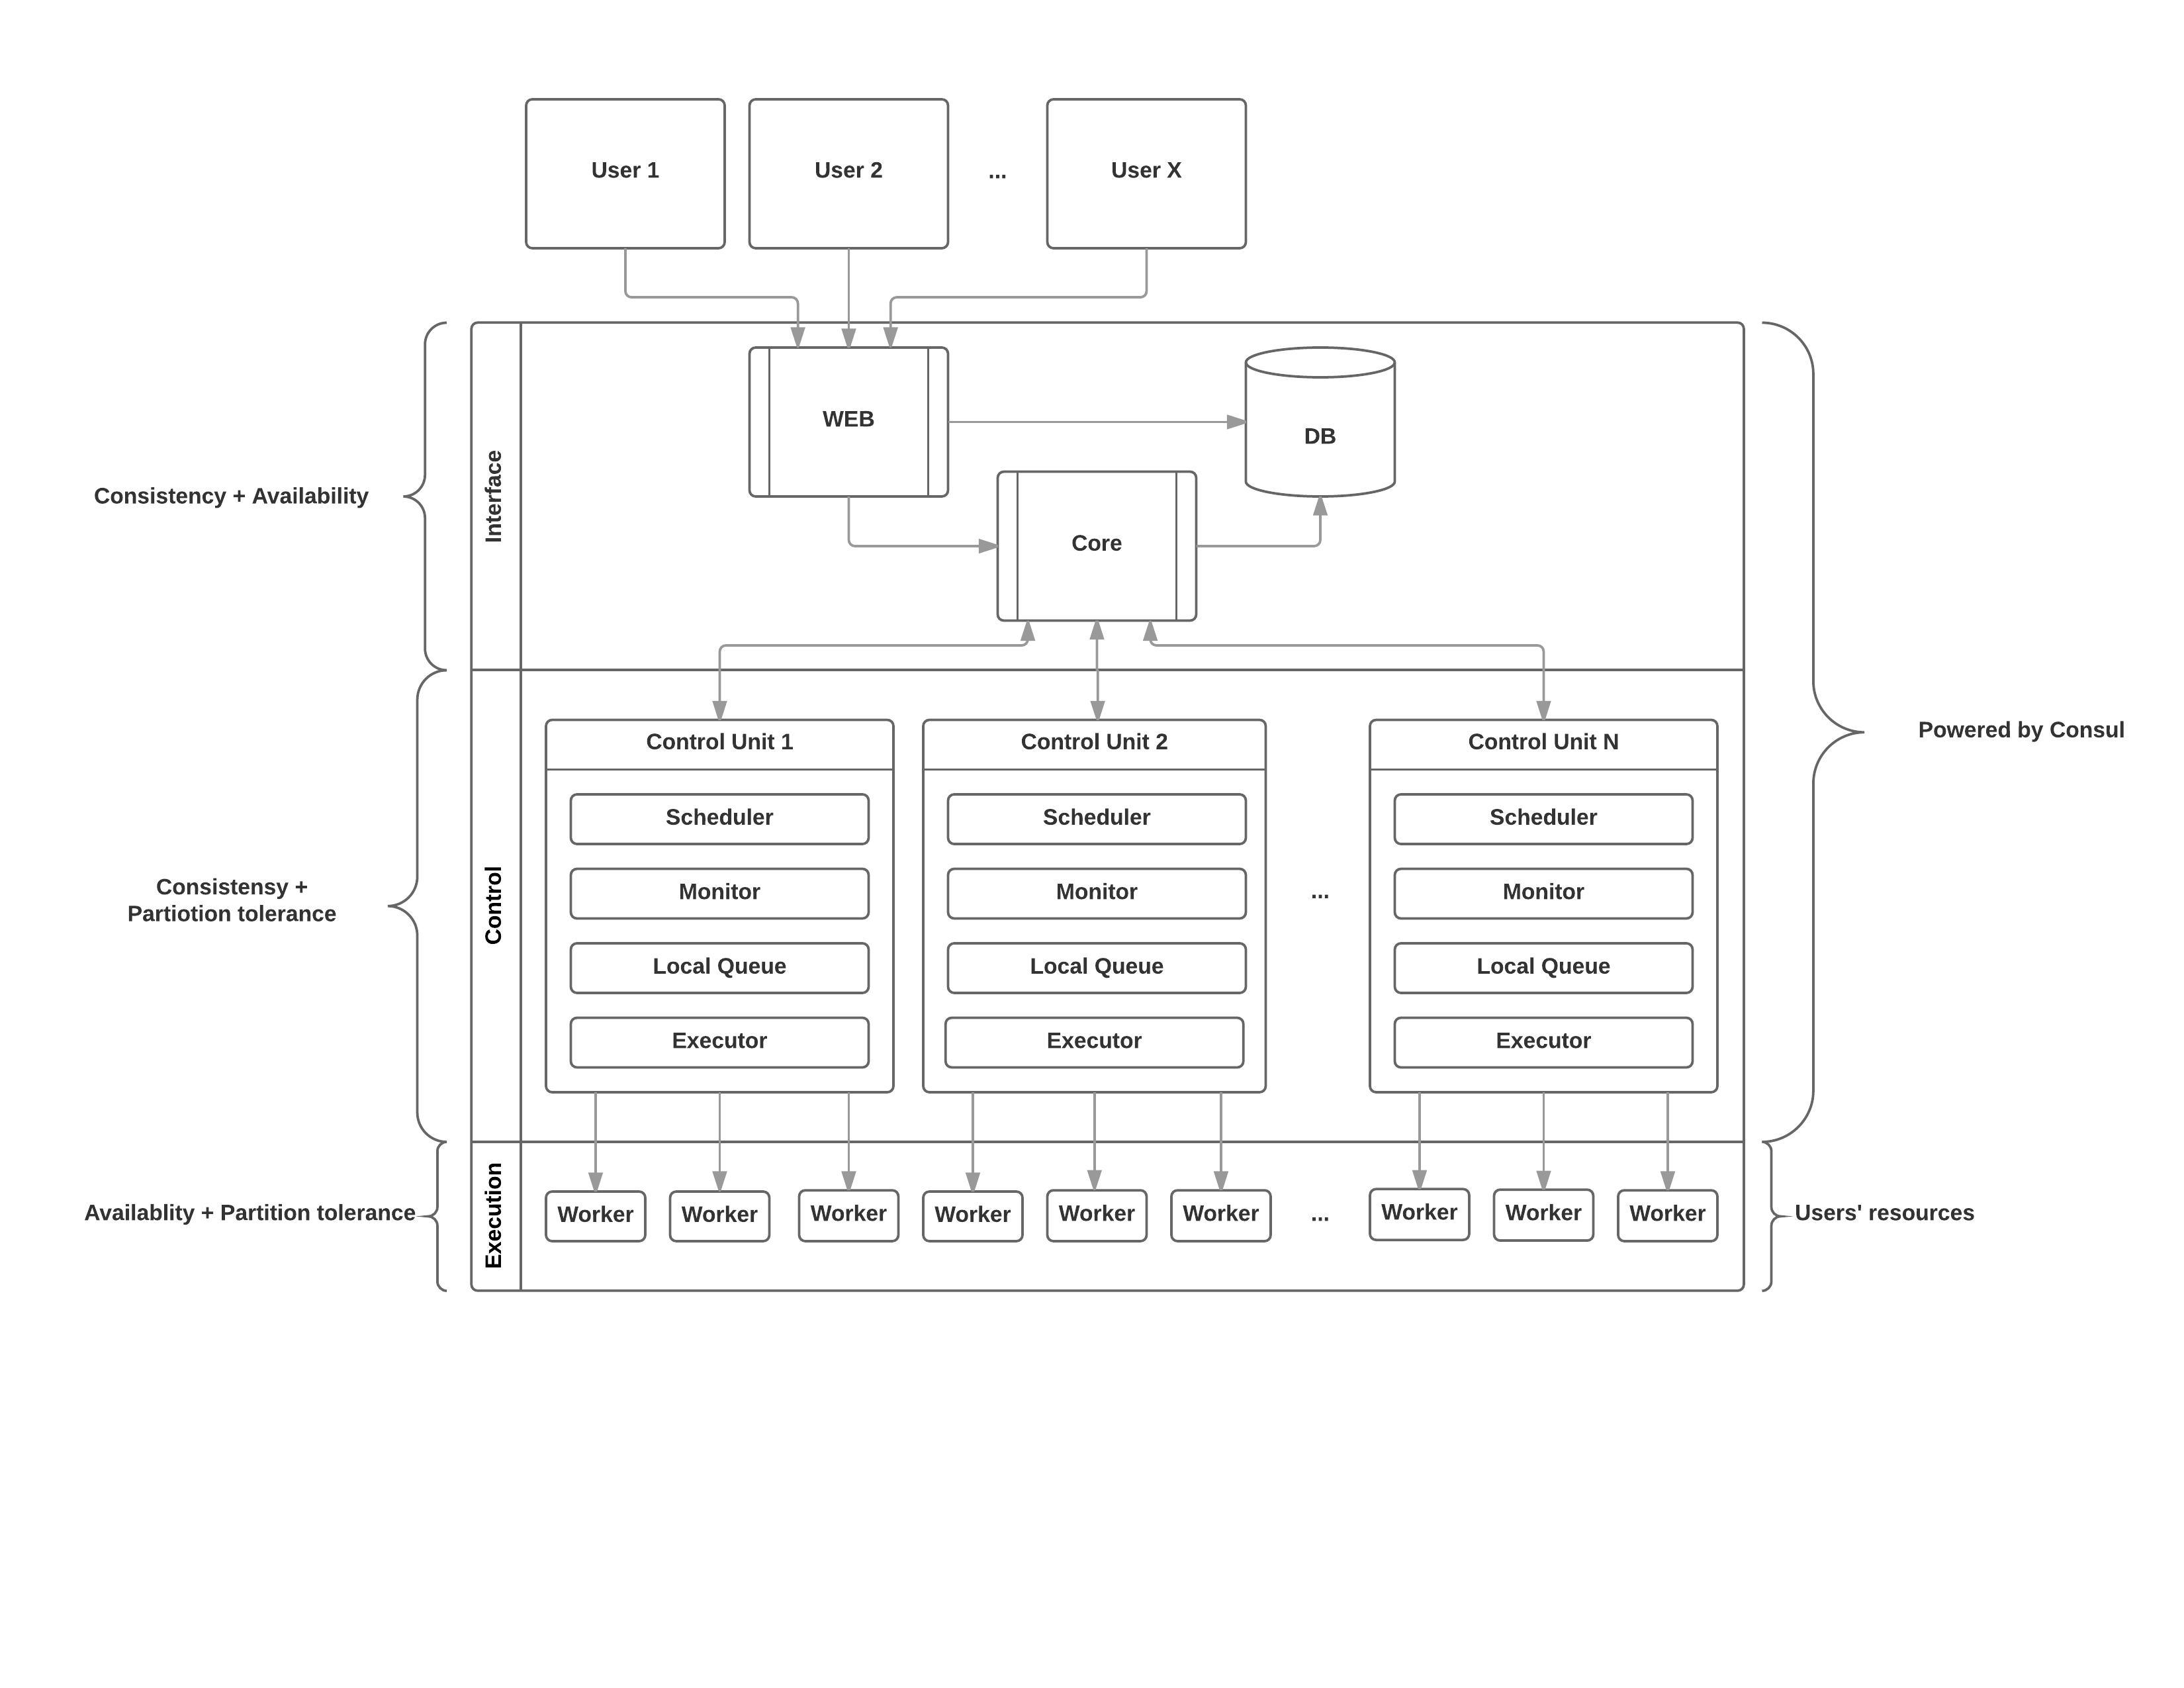
\includegraphics[width=\textwidth]{fig/architecture}
	\caption{Диаграмма архитектуры}\label{fig:architecture}
\end{figure}

Но для начала объясню общую структуру. Здесь видно разделение на три слоя плюс пользователи системы. User 1 -- User X - это пользователи из категорий исследователей и гостей. Каждый слой состоит из компонентов. Распределение компонентов по машинам специфично для каждого слоя. Для слоя Interface оно явно не ограничивается предложенной архитектурой. В зависимости от нагрузки и прочих факторов все эти компоненты могут быть как на одной машине, так и разнесены по нескольким. Для слоя Control истинно правило "одна машина - один Control Unit". Для слоя Execution все просто - один Worker равен одной машине предоставленной для вычислений.

Направление стрелок - это кто кому шлет запросы или кто является инициатором долговременного соединения.

Первые два слоя - это “наши” машины, которым мы доверяем и только у нас есть к ним доступ.

Третий слой - машины предоставленные извне, мы им “не доверяем”.

Слева показаны приоритеты в терминах CAP-теоремы для каждого слоя.

\subsection{Слой Execution}

На этом слое находятся машины, предоставленные пользователями системы. Они частично конфигурируются нами и не содержат никакого кода, который бы управлял слоями выше (из соображений безопасности). Про специфику работы с этими ресурсами было написано выше.

Все запросы приходят со слоя Control.

\subsection{Слой Control}

Состоит только из Control Unit’ов. Каждый Control Unit - это отдельная машина. Каждый Worker из слоя ниже принадлежит только одному Сontrol Unit’y.

Control Unit состоит из нескольких логических компонент и представляет из себя монолитную программу.

Все Control Unit с этого слоя представляют из себя распределенную систему. То есть запросы с верхнего слоя Interface по своей сути направлены не к конкретному Control Unit'у, а ко всей системе целиком.

Смысл подобного разбиения - это большая стабильность системы. Т. е. эффективным подходом будет, например, по одному Control Unit на географическую зону.

Смысл всей этой системы в следующем:

\begin{itemize}
	\item Получать задания со слоя выше (от Сore)
	\item Раскидывать датасеты по Worker’ам
	\item Запускать вычисления на Worker’ах
	\item Отправлять результаты вычислений на Worker’ах на слой выше (в Core).
\end{itemize}

Теперь конкретные примеры запросов, которые могут приходить в эту систему:

\begin{itemize}
	\item Загрузи датасет
	\item Загрузи и собери этот docker-контейнер
	\item Обнови этот докер контейнер
	\item Обнови этот датасет
	\item Запусти этот контейнер с этим датасетом
\end{itemize}

Из подобных задач формируются локальные очереди (Local Queue). В какую локальную очередь и на какой Worker отправить задачу определяет “распределенный” Scheduler. Также состояние, корректность и доступность Worker'ов, прочие глобальные характеристики системы отслеживаются Monitor'ом. Monitor может давать информацию о всех доступных Worker'ах системы. Monitor - основной инструмент Scheduler'а для получения текущего состояния системы. Executor отвечает за "опустошение" очереди и выполнение задач на Worker'ах.

Результат выполнения работы отправляется в Core, который, в свою очередь, решает где хранить этот результат.

\subsection{Слой Interface}

Распределение по машинам в этом слое диктуется лишь нагрузкой. При малом количестве пользователей - можно все три компонента держать на одной машине. Теперь отдельно про каждый компонент.

\begin{description}
  \item[WEB] Веб-приложение написанное на любом адекватном web-фреймворке. Именно через него происходит постановка задач, просмотр результатов и прочее. Является единой точкой управления системой как для рядовых пользователей, так и для администраторов. Важно понимать, что тут не только HTML + JS, но и реализована вся бизнес-логика интерфейса.
  \item[DB] Основная база данных. В ней хранится как все относящееся к бизнес-логике приложения. По своему содержанию должна быть независима от нижестоящих слоев. Т. е. если конфигурация всего того, что есть ниже станет иной - данные не должны стать некорректными.
  \item[Core] WEB не общается напрямую со слоем Сontrol. Он работает с Core через API, а оно в свою очередь контролирует слой ниже. Т. е. Core - это микросервис взаимодействия со слоем Control.
\end{description}


\section{Выбор технологий для реализаций компонентов}

Сначала надо определить "сколько переменных в уравнении".

Во первых стоит определиться с WEB. Поскольку почти вся бизнес-логика сконцентрирована в этом компоненте, надо работать с HTML/JS, реализовывать пользовательский интерфейс, интегрировать платежные системы и прочее - то получается, что требования к инструменту реализации этого компонента стоят особняком от прочих.

Потом идет DB. Здесь все просто - надо выбрать подходящую основную базу данных.

Worker'ы - здесь нет никаких программных решений, только технические требования.

А вот Control Unit и Core компоненты имеет смысл реализовывать одной технологией. Причем здесь оправдано использование чего-то отличного от выбранного для WEB-компонента ибо спектр задач существенно отличается. Решая задачу правильным инструментом мы экономим время и деньги.

Итого нам нужно принять три решения: что использовать для написания WEB, что использовать для написания Core и Control Unit, что использовать в качестве основной БД.

\subsection{WEB}

Написанное ниже имеет рекомендательный характер. Если будет использована какая-либо другая технология - это никак не скажется на проведенной мной работе.

Основное занятие автора этой работы - веб-разработка сложных проектов на Ruby on Rails. Мнения изложенные ниже основываются на моем личном опыте и общим наблюдением за рынком.

Посколько Evergrid является по своей сути стартапом, то важным аспектом является скорость разработки. То есть надо быть быстро создать прототип и иметь возможно быстро вносить изменения. На Java и ASP.NET подобное получается плохо, особенно у небольших команд. Наиболее успешно используемые технологии это Ruby on Rails, Node.js, Django и прочие python-фреймворки, PHP.

По возможности я бы не советовал брать Node.js или PHP - обе эти технологии страдают от плохого дизайна языка. Ruby и Python гораздо более удачно спроектированные языки и могут одинаково хорошо подойти для решения поставленной задачи. Конечно, можно плохо писать код на любом языке, но по моему мнению это несколько сложнее делать на Ruby и Python. К тому же что для Rails, что для Django есть огромное количество готовых решений типовых проблем в виде библиотек. По этому параметру Rails даже опережает Django, но если уже есть люди знающие Python и готовые писать проект - это недостаточная причина чтобы заставлять их учить новый язык программирования.

Но что у Python, что у Ruby есть недостаток. Это относительно низкая скорость, синхронная архитектура предпочтительных веб-фреймворков, GIL и никакого статического анализа на этапе компиляции т. к. этапа компиляции нет. Эти недостатки могут оказаться критичными если ожидается большой наплыв пользователей на раннем этапе. Но использование enterprise-технологий вроде Java и ASP.NET не единственный возможный выход из ситуации. Есть два хороших кандидата: Play Framework (написанный на Scala) и Phoenix Framework (написанный на Elixir).

Play Framework уже активно используется и его можно считать за production-ready решение. Высокая стабильность обеспечивается сильной системой типов языка Scala и тем, что он основан на реализации акторной модели Akka. Имеет высокую производительность по сравнению с Rails/Django и асинхронную архитектуру.

Phoenix Framework моложе чем Play, на данный момент менее распространен и язык, на котором он написан (Elixir) моложе чем Scala. Стабильность обеспечивается тем, что Elixir - это язык для BEAM (Erlang VM) с полной поддержкой OTP и библиотек из Erlang. А Erlang/OTP известны своей исключительной стабильностью. Несмотря на то, что это язык с динамической типизацией компилятор в байткод машины делает большое количество проверок (в том числе и касающихся системы типов), что помогает отлавливать многие ошибки уже на этом этапе.

\subsection{Core и Control Unit}

Эти два компонента формируют внутреннюю инфраструктуру сервиса. В данном случае корректным будет следующий список требований:

\begin{itemize}
	\item высокая производительность (система должна адекватно вести себя под высокими нагрузками)
	\item выбранное решение должно использоваться для схожих известных продуктов
	\item иметь развитые библиотеки для сетевого взаимодействия
	\item чем проще будет инициализировать новые сервера - тем лучше
	\item язык должен быть популярен и иметь активное сообщество
\end{itemize}

Требование высокой производительности ставит под сомнение использование интерпретируемых языков. Из "быстрых" языков в первую очередь приходят на ум C/C++ и go. ASP.NET плохо дружит с Linux, а Java/Scala довольно прожорливы в плане памяти. Если внимательнее посмотреть на go, то становится видно, что он является хорошим решением.

На нем написаны продукты hashicorp (nomad, consul), на нем написан docker. Он быстр. Он проще C/C++. На нем активно пишут всяческие сервисы. И последнее, но не последнее по важности: он прост в изучении. Опытный программист может освоится и начать писать на нем спустя два-три вечера изучения.

Более того, благодаря встроенной в язык модели параллелизма CSP писать параллельный и конкурентный код на нем существенно проще чем на C/C++.


\subsection{DB}

На самом деле на данном этапе сложно предсказать все те требования, которые могут возникнуть для основного хранилища. Возможно, даже одного продукта не хватит и будет использоваться некая комбинация (например: часто можно встретить связки Postgres + Redis).

Но в качестве решения по умолчанию стоит рассматривать именно Postgres. На данный момент это наиболее универсальное и активно используемое решение среди open source баз данных.

\section{Аспекты реализации инфраструктуры. CAP-теорема}

Поскольку мы имеем дело с распределенной системой то стоит явно указать приоритеты в терминах CAP-теоремы. Причем эти приоритеты отдельные для каждого слоя (именно из-за этого вообще появилось разделение на слои).

Также первый и второй слой используют consul - он предоставляет service discovery и leader election интерфейсы, к тому же он создан для решения этих задач как раз таки в распределенных системах.

%\textit{Сформулировать CAP-теорему.}

%\textit{Hashicorp consul}

\begin{description}
  \item[Слой Execution] Для этого слоя подходит конфигурация [C]AP. Если машина отвалилась и не поднимается -- перераспределяем нагрузку. Здесь важно в любой момент времени максимально использовать доступные ресурсы.
  \item[Слой Control] При критичной сегментации сети в слое, Control Unit'ы перестают принимать запросы, но продолжают выполнение локальных очередей. Примерно так выглядит жертва availability во имя consistency и partition tolerance.
  \item[Слой Interface] На этом слое крайне важна согласованность данных, а без доступности он не имеет смысла. Поэтому жертвуем partition tolerance.

\end{description}
